\section{Audit and exploratory findings}
\begin{table}[htbp]\centering
\caption{Observed source and analytical sample.}\label{tab:audit}
\begin{tabular}{lr}\toprule
Quantity & Count / range\\\midrule
Raw transaction lines & 2,595,732\\
Product records & 92,353\\
Observed households & 2,500\\
Observed day indices & 1--711\\
Excluded nonpositive quantity or sales lines & 18,917\\
Retained positive purchase lines & 2,576,815\\
Calibration lines (day $\leq500$) & 1,726,165\\
Later lines (day $>500$) & 850,650\\
Calibration household cohort & 2,498\\
Later-only households outside cohort & 2\\
Cohort households with no later purchase & 59\\\bottomrule
\end{tabular}\end{table}
The transaction table has 12 columns and the product table seven. Both required tables contain zero missing cells under the CSV parser, no exact duplicate transaction rows and no duplicate product keys. All purchased product identifiers match the product table; the join preserves the transaction row count. Basket identifiers have neither conflicting household assignments nor conflicting day assignments. The eight-file schema inventory also verifies UTF-8-compatible decoding of the complete byte streams and records column names and sampled types. Only transactions and products enter clustering; demographics and campaign tables are intentionally not joined. These checks support the household aggregation and rule out join multiplication.

There are 14,466 nonpositive-quantity lines and 18,850 nonpositive-sales lines; their union is 18,917, or 0.73\% of raw lines. These counts overlap. Negative retail discounts occur on 1,303,026 lines and are retained and used only to construct the negative-discount indicator. The calibration covers days 1--500; the later period covers days 501--711. Because the windows differ in length, calibration and later totals are not comparable as growth rates.

\begin{figure}[htbp]\centering
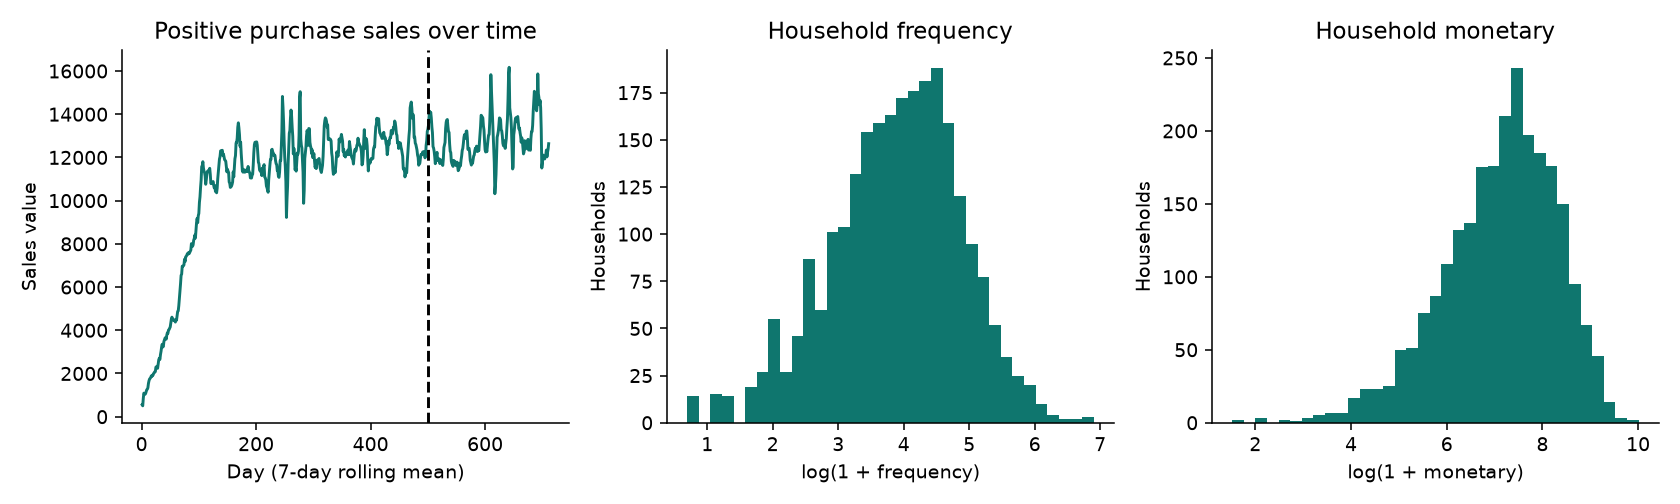
\includegraphics[width=\textwidth]{../figures/01_eda.png}
\caption{Recorded positive-purchase sales and household activity distributions. The dashed temporal boundary marks the calibration/later split on the exact day scale. Household activity is displayed after a log transform because raw purchase intensity is strongly heterogeneous.}\label{fig:eda}
\end{figure}
The EDA motivates a baseline focused on shopping intensity in a transformed distance space. Monetary value and frequency are related because more shopping occasions give more opportunities to spend. Basket-level and assortment measures may repeat the same intensity signal, whereas department shares add preference information directly. The selected eight departments are Grocery, Drug GM, Produce, Meat, Kiosk-Gas, Meat-Packaged, Deli and Pastry.

\section{Model comparisons}
\subsection{Within-space selection}
All three representative K-means models select two clusters under the predeclared minimum-size and silhouette rule. The RFM groups contain 882 and 1,616 households; Behavior contains 809 and 1,689; Product contains 843 and 1,655. These are substantial groups rather than isolated outlier collections.

\begin{table}[htbp]\centering
\caption{Selected K-means models. Silhouette and Davies--Bouldin (DB) values are measured in each model's own space; they do not establish a cross-space ranking.}\label{tab:selected}
\begin{tabular}{lrrrrr}\toprule
Space & Dimensions & $k$ & Smallest group & Silhouette & DB\\\midrule
RFM &3&2&882&0.456&0.857\\
Behavior &8&2&809&0.329&1.237\\
Product &17&2&843&0.206&1.984\\\bottomrule
\end{tabular}\end{table}
\begin{figure}[htbp]\centering
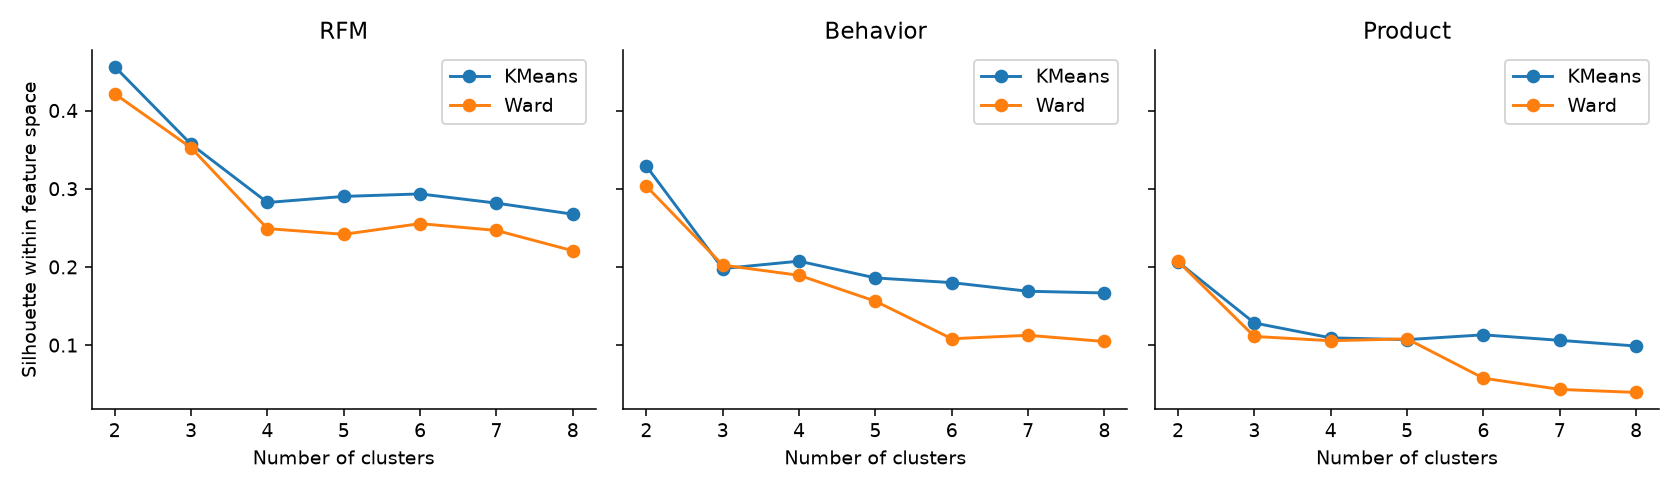
\includegraphics[width=\textwidth]{../figures/02_model_selection.png}
\caption{Candidate K-means and Ward silhouette curves. Compare cluster counts and algorithms within a panel; each panel defines its own distance space.}\label{fig:selection}
\end{figure}
Two groups offer the strongest within-space K-means separation among eligible candidates. Two clusters summarize a continuous intensity gradient rather than two intrinsic household types.

The tested DBSCAN grid does not produce a compelling full-cohort alternative. In RFM at the 70th-percentile neighborhood setting, two groups remain after 18.2\% of households are marked noise, with silhouette 0.162 on retained rows. At tighter settings it yields six groups and negative silhouette. In Behavior, the only two-group setting has a group of just eight households and 14.2\% noise. All tested Product settings produce one non-noise cluster, making multi-cluster silhouette undefined.

\subsection{Stability and partition agreement}
\begin{table}[htbp]\centering\small
\caption{ARI stability. Subsample columns summarize 20 paired independent 80\% samples; reported ranges are empirical minima and maxima, not confidence intervals.}\label{tab:stability}
\begin{tabular}{lrrrr}\toprule
 &\multicolumn{2}{c}{K-means subsamples}&\multicolumn{2}{c}{Ward subsamples}\\
Space & Mean & Range & Mean & Range\\\midrule
RFM &0.980&0.948--1.000&0.535&0.011--0.874\\
Behavior &0.970&0.923--0.995&0.457&0.154--0.740\\
Product &0.964&0.860--0.990&0.314&$-0.024$--0.584\\\bottomrule
\end{tabular}\end{table}
\begin{figure}[htbp]\centering
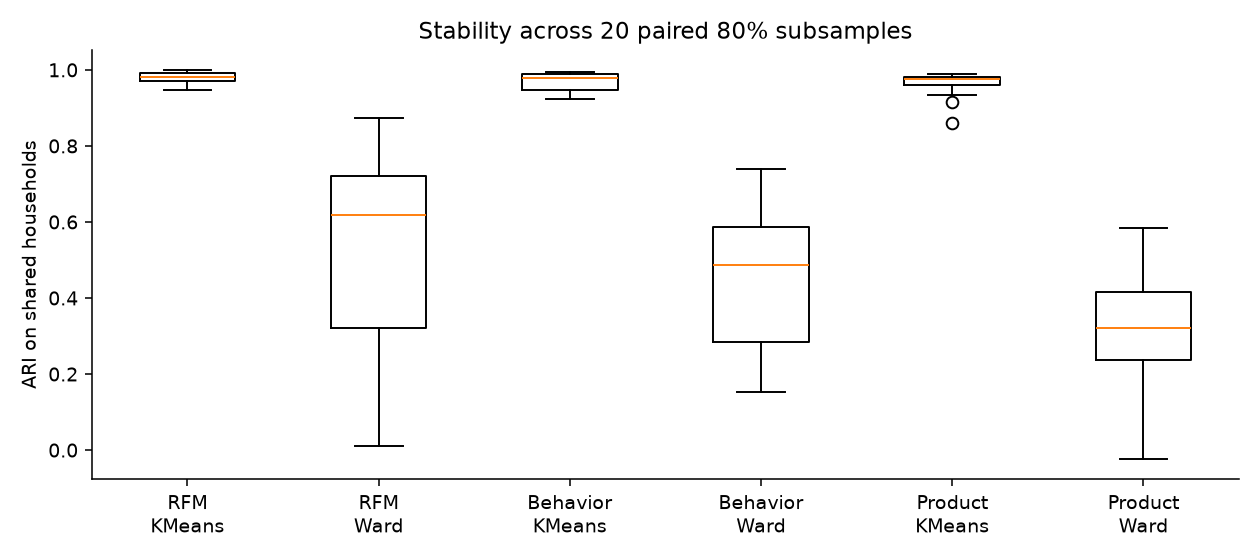
\includegraphics[width=.94\textwidth]{../figures/03_stability.png}
\caption{Conditional sampling stability on shared households. The K-means partitions are substantially more reproducible than Ward under this perturbation.}\label{fig:stability}
\end{figure}
Mean one-initialization ARI against the selected K-means fit is 0.994 for RFM, 0.982 for Behavior and 0.997 for Product. The main findings do not depend on one random start. K-means sampling stability remains high in all three spaces; Product's minimum subsample agreement is lower, so the additional representation does not improve robustness. Ward is substantially more sensitive to household sampling, especially in Product space. K-means is the more reproducible method.

Across selected partitions, RFM--Behavior ARI is 0.614, RFM--Product is 0.589 and Behavior--Product is 0.850. Enrichment changes some assignments, and Product is much closer to Behavior than RFM. Assignment change matters only if it reveals useful new profile distinctions. Numeric cluster identifiers are space-specific; Product cluster 0 corresponds to the higher-activity group, whereas the higher-activity RFM and Behavior group is numbered 1.

\section{Profiles and later-period descriptive checks}
\begin{table}[htbp]\centering\small
\caption{Calibration profiles in original units. Means are descriptive household averages. H and L denote higher- and lower-activity groups within a space, not common fixed memberships.}\label{tab:profiles}
\begin{tabular}{llrrrr}\toprule
Space & Group & $n$ & Recency (days) & Baskets & Recorded sales\\\midrule
RFM &L&882&67.9&20.8&507.7\\
RFM &H&1,616&6.2&104.4&3,034.0\\
Behavior &L&809&68.9&23.8&418.1\\
Behavior &H&1,689&8.4&99.4&2,967.7\\
Product &L&843&65.8&25.5&448.4\\
Product &H&1,655&8.7&100.1&3,004.7\\\bottomrule
\end{tabular}\end{table}
All representations chiefly separate higher-intensity, recently active households from less-frequent and less-recent households. In Product, higher-activity households average 549.7 distinct products and 12.8 departments, versus 114.1 products and 7.6 departments in the lower-activity group. They also have larger mean baskets (35.6 versus 23.0 sales units). Discount-line proportions are close (50.4\% versus 48.9\%), so the two groups are not distinct discount-response types.

\begin{figure}[htbp]\centering
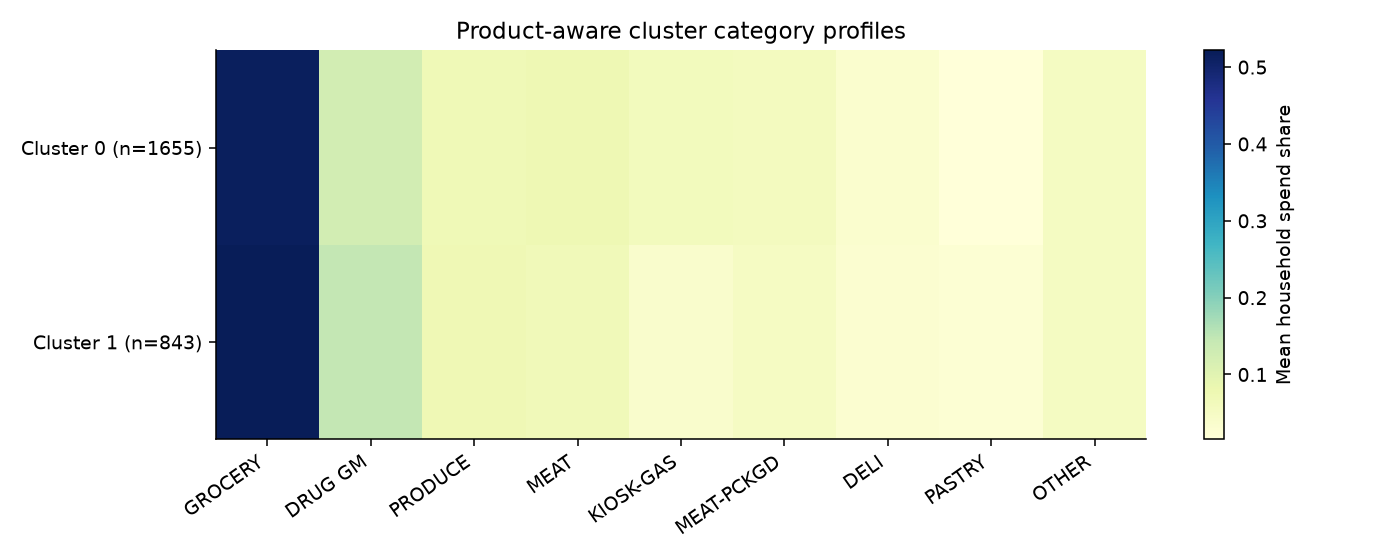
\includegraphics[width=\textwidth]{../figures/04_category_profiles.png}
\caption{Product-aware department profiles: mean of household spend shares, rather than a share of pooled group revenue. Grocery dominates both groups; the modest contrasts qualify how much preference-specific structure the two-group solution reveals.}\label{fig:composition}
\end{figure}
Both Product groups allocate about half of spending to Grocery (51.4\% in the higher-activity group and 52.2\% in the lower). The higher-activity group has a greater Kiosk-Gas share (6.0\% versus 3.7\%) and Meat share (7.5\% versus 6.6\%), while the lower-activity group has more Drug GM (14.5\% versus 12.3\%) and Pastry (2.4\% versus 1.6\%). These differences are useful descriptions but small in absolute terms.

\begin{table}[htbp]\centering\small
\caption{Later-period positive-purchase sales by frozen group. Brackets are 95\% percentile bootstrap intervals for group means, conditional on the fixed clustering; activity is the proportion with any observed later purchase.}\label{tab:later}
\begin{tabular}{llrrr}\toprule
Space & Group & Mean later sales [interval] & Later active & $\eta^2$\\\midrule
RFM &L&343.2 [318.3, 371.2]&93.9\%&0.204\\
RFM &H&1,487.5 [1,424.0, 1,547.0]&99.7\%&\\
Behavior &L&306.3 [280.7, 332.1]&93.7\%&0.197\\
Behavior &H&1,455.7 [1,393.7, 1,516.8]&99.5\%&\\
Product &L&320.8 [297.6, 347.1]&94.1\%&0.202\\
Product &H&1,471.9 [1,413.7, 1,535.6]&99.5\%&\\\bottomrule
\end{tabular}\end{table}
\begin{figure}[htbp]\centering
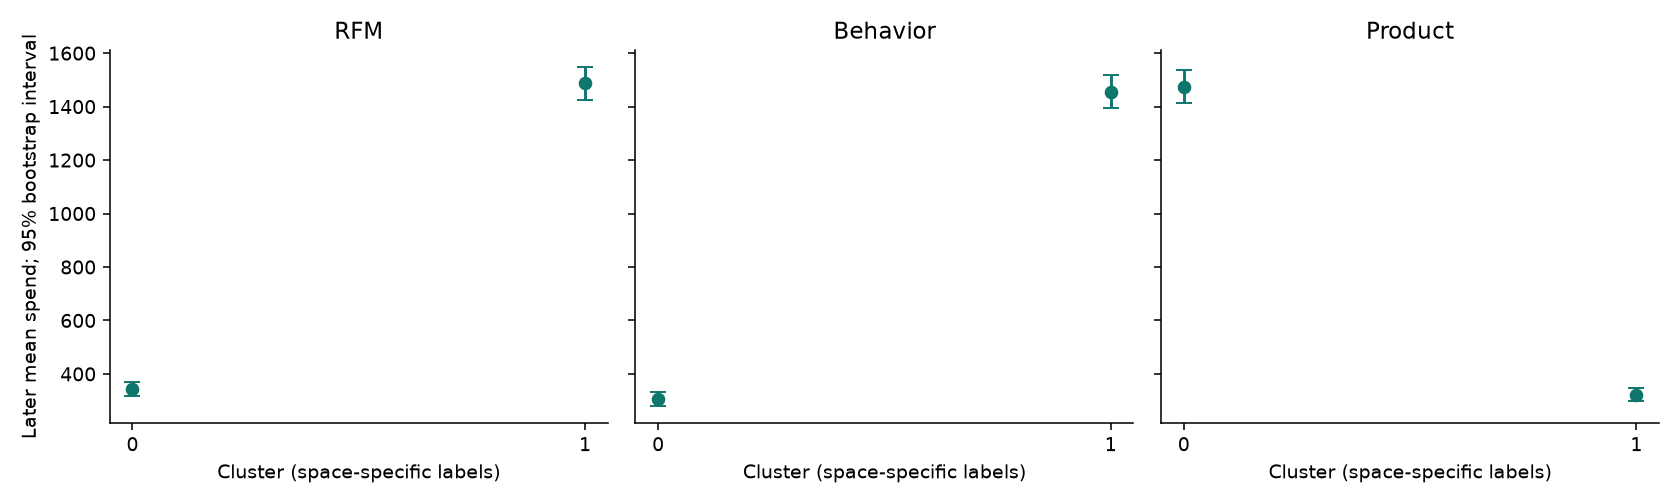
\includegraphics[width=\textwidth]{../figures/05_holdout.png}
\caption{Later mean spending and bootstrap uncertainty. Calibration-defined groups remain descriptively different, with much larger within-cohort purchase intensity in the higher-activity group. Labels are independent in each panel.}\label{fig:holdout}
\end{figure}
The frozen groups retain a large later-period spending difference. Nevertheless, Product explains 20.2\% of later spend variance, compared with 20.4\% for RFM and 19.7\% for Behavior. The absolute Product--RFM difference is approximately $-0.002$ in $\eta^2$. Product therefore brings no improvement on this criterion, and most variance remains within groups.

The intervals reflect group-mean uncertainty, not the uncertainty of a difference between representations. Because the models use the same households, a paired household bootstrap of Product-minus-RFM explained variance gives $-0.00190$, with a conditional 95\% interval $[-0.01426,0.00860]$. This provides no clear evidence of improvement. Holdout results were not used in model selection.


